% Fig. 2.11 / spec Fig A10 + A11 -- same expectation, different variance.
% Source: mathstatch2.tex lines 1653-1690 and 1692-1729, two separate
%   tikzpictures which spec 3.2 item 7 rules must become one picture: the two
%   manuscript curves enclose 2.506628 and 1.754744 of area, so comparing
%   their spreads is misleading, and the second one is only drawn over 2:4.
%
% This file replaces a hand-written SVG (720 x 380 user units, not a pdflatex
% product).  Three faults of that file are fixed here:
%   - its four type sizes came to 10.2 / 9.7 / 9.2 / 6.8px at a 350px display
%     width, none of them reaching the 12px floor of spec 1.3;
%   - it carried Chinese inside the picture, against spec 1.4;
%   - its two curves were told apart by hue alone (#9c2d2d against #6f7d65),
%     against spec 1.7.
%
% Densities, both centred on 3 and both integrating to 1:
%   solid  N(3, 1)     f(x) = 0.3989423 exp(-(x-3)^2/2),   peak 0.3989423
%   dashed N(3, 0.5^2) f(x) = 0.7978846 exp(-2(x-3)^2),    peak 0.7978846
% At y = 3.6cm the peaks stand 1.4362cm and 2.8724cm high, as spec A11 sets
% out.  The narrow curve is plotted over 1:5 only: outside that range its
% density is under 0.00027 (0.001cm, indistinguishable from the axis) and
% pgfmath cannot represent exp(-18) anyway.
%
% Deviations from CH2_FIGURE_SPECS.md:
%
% 1. The Chinese labels of the old SVG ("larger variance", "smaller variance",
%    "the same expectation") are gone, as spec 1.4 requires.  Their work is
%    done by the two curve labels sigma^2 = 1 and sigma^2 = 0.25 and by the
%    caption, which has to name both distributions.
%
% 2. Per spec 1.9 the two curves carry two independent cues: line style
%    (solid against dash pattern on 4pt off 2pt) and a label written at the
%    curve itself.  Colour is no longer a cue; both curves are journalink.
%
% 3. The old SVG filled the area under each curve (opacity 0.14 and 0.18 in
%    two different hues).  The fills are dropped: in a single accent colour
%    two overlapping fills would read as three bands of tint, and the fills
%    carry no information here, the figure being about spread rather than
%    about any particular probability.  Spec 1.2 caps fill opacity but does
%    not require a fill.
%
% 4. \DeclareMathSizes{10}{10}{9}{8} raises the math script sizes from the
%    default 7pt/5pt, so that the exponent of sigma^2 and the X of mu_X also
%    clear the floor.  Native size 219.042 x 106.055 pt (drawing range 7.59cm
%    wide, inside the 9.0cm cap of spec 1.3); a mark of S pt shows at
%    S x 0.99626 x <display width> / 219.042 px, so at the 350px phone width
%    measured for P208
%        10pt text 15.9px, 9pt scripts 14.3px, 8pt scriptscripts 12.7px
%    and at the 620px desktop width 28.2 / 25.4 / 22.6px.
%    The x scale is 1.12cm per unit rather than a round 1cm precisely so that
%    the scriptscript size clears 12.5px at 350px.
%    This is the same declaration already used in quartiles-equal-areas.tex;
%    it is not the site-wide \sssig change that ruling 21 defers.
\documentclass[tikz,border=2pt]{standalone}
\usepackage{amsmath}
\usepackage{amssymb}
\usepackage{xcolor}
\usetikzlibrary{arrows.meta}
\newcommand{\sssig}{\scriptscriptstyle}
\DeclareMathSizes{10}{10}{9}{8}

\definecolor{journalink}{HTML}{1F1C18}
\definecolor{journalmuted}{HTML}{8A7F72}
\definecolor{journalaccent}{HTML}{9C2D2D}

\begin{document}
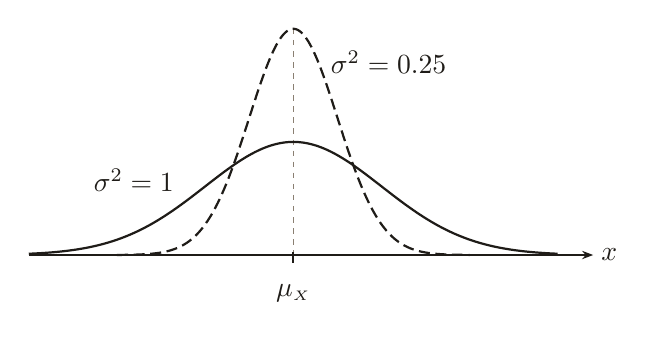
\begin{tikzpicture}[
  x=1.12cm,
  y=3.6cm,
  every node/.style={font=\normalsize, journalink},
  axis/.style={journalink, line width=0.8pt, -{Stealth[length=4pt]}},
  tick/.style={journalink, line width=0.8pt},
  wide/.style={journalink, line width=0.8pt},
  narrow/.style={journalink, line width=0.8pt, dash pattern=on 4pt off 2pt},
  guide/.style={journalmuted, line width=0.5pt, dash pattern=on 2pt off 2pt}
]
  % ---- x axis ----------------------------------------------------------
  \draw[axis] (0,0) -- (6.4,0);
  \node[anchor=west, inner sep=2.8pt] at (6.4,0) {$x$};

  % ---- the common expectation ------------------------------------------
  \draw[guide] (3,0.7978846) -- (3,0);
  \draw[tick] ([yshift=0.035cm]3,0) -- ([yshift=-0.106cm]3,0);
  \node[anchor=north] at ([yshift=-0.25cm]3,0) {$\mu_{\sssig X}$};

  % ---- N(3,1): the wider spread, solid ---------------------------------
  \draw[wide] plot[domain=0:6, samples=200, smooth]
    (\x,{0.3989423*exp(-(\x-3)*(\x-3)/2)});
  \node[anchor=south east, inner sep=0pt] at ([yshift=0.80cm]1.65,0)
    {$\sigma^{2}=1$};

  % ---- N(3,0.5^2): the tighter spread, dashed --------------------------
  \draw[narrow] plot[domain=1:5, samples=200, smooth]
    (\x,{0.7978846*exp(-2*(\x-3)*(\x-3))});
  \node[anchor=west, inner sep=0pt] at ([yshift=2.45cm]3.42,0)
    {$\sigma^{2}=0.25$};
\end{tikzpicture}
\end{document}
